\documentclass[25pt, a0paper, portrait]{tikzposter}

%Вставка картинок
\usepackage{graphicx}
\graphicspath{}
\DeclareGraphicsExtensions{.pdf,.png,.jpg,.jpeg}

%Таблицы
% \usepackage[table,xcdraw]{xcolor}
% Cсылки
\usepackage{hyperref}
\bibliographystyle{unsrt}
%Математика
\usepackage{amsmath, amsfonts, amssymb, amsthm, mathtools }
\DeclareMathOperator*{\Res}{Res}
\DeclareMathOperator*{\sign}{sign}
\DeclareMathOperator*{\Real}{Re}
\DeclareMathOperator*{\Imag}{Im}
\newcommand{\groupn}{\mathbb{Z}_n}

%%Окружение для многострочных уравнений
\newenvironment{eqw}{\begin{equation} \begin{aligned}}   
    {\end{aligned}    \end{equation}}
\newenvironment{eqw*}{\begin{equation*} \begin{aligned}}   
    {\end{aligned}    \end{equation*}}

% for tikz
\usepackage{pgfplots}
\usepackage{physics}
\usepackage{tikz}
\pgfplotsset{compat=1.15}
\usepackage{mathrsfs}
\usetikzlibrary{arrows}
% from overleaf
\usepackage{blindtext}
\usepackage{comment}
%table env
\newcounter{tablecounter}
\newenvironment{tikztable}[1][]{
  \def \rememberparameter{#1}
  \vspace{7mm}
  \refstepcounter{tablecounter}
  \begin{center}
  }{
    \ifx\rememberparameter\@empty
    \else %nothing
    \\[10pt]
    {\rememberparameter}
    \fi
  \end{center}
  \vspace{7mm}
}

\title{Quasiprobability distributions of bright ''banana'' states}
\author{Bulat Nugmanov}
\institute{RQC / MIPT}

\usetheme{Board}

\begin{document}
\maketitle

\begin{columns}
\column{0.4}
\block{Problem statement}
{
    We start with the following Hamiltonian:
    \begin{equation*}
        \hat{H}_{Kerr} = \hbar \omega \hat{a}^{\dagger}\hat{a} + \hbar\gamma \hat{a}^{\dagger2}\hat{a}^{2}
    \end{equation*}
    And let's study the evolution of the coherent state $\ket{\alpha}$:
    \begin{equation*}
        \ket{\psi} = e^{-\frac{i}{\hbar} \hat{H}_{Kerr} \tau} \ket{\alpha} \sim \frac{e^{-\frac{\abs{\alpha}^2}{2}}}{\pi^{1/4}} 
        \sum\limits_{n=0}^{\infty}\frac{\alpha^n}{\sqrt{n!}}e^{i\Gamma n^2}\ket{n}
    \end{equation*}
    The main parametrs have the following orders:
    \begin{equation*}
    \left\{
    \begin{aligned}
        \gamma\tau = \abs{\Gamma}&\sim 10^{-6}\\
        \abs{\alpha}^2&\sim 10^{+6}
    \end{aligned}
    \right.
    \end{equation*}
    The state $\ket{\psi}$ we study using Husimi and Wigner functions:
    \begin{equation*}
    \begin{aligned}
        Q(\beta) = \frac{\left|\langle\psi |\beta\rangle\right|^2}{\pi} =
        \frac{e^{-|\alpha|^2-|\beta|^2}}{\pi}\left|
        \sum\limits_{n = 0}^{\infty}\dfrac{\left(\alpha \beta^*\right)^n e^{-i \Gamma n(n-1)}}{n!}\right|^2\\
        W(\beta)=\frac{1}{\pi}\int\limits_{-\infty}^{\infty}dy\, \psi^*(\Real\beta+y)\psi(\Real \beta-y)e^{2ip\Imag \beta}
    \end{aligned}
    \end{equation*}
    They have the following connection via Fourier transform:
    \begin{equation*}
        C_s(z) = \mathcal{F}\left\{W\right\}(z) = e^{\frac{\abs{z}^2}{2}} \mathcal{F}\left\{Q\right\}(z) = e^{\frac{\abs{z}^2}{2}} C_a(z)
    \end{equation*}
    \textit{The main problem is to calculate this quasi-probabilistic functions in a reasonable time.}
    \innerblock{Table of nonlinearities}
    {
        \begin{tikztable}
            [The best performance archived for cubically nonlinear media in microresonators. $\Gamma = \gamma \tau$ is defined by archived quality with non-linearity determined by the material.]
            \centering
            \begin{tabular}{|c|c|c|c|}
                \hline
                % \rowcolor[HTML]{EFEFEF} 
                Material        & $Q$              & $\gamma$, Hz & $\Gamma\cdot10^{-6}$ \\ \hline
                Al$_2$O$_3$     & $2\times10^9$    & 0.06         & 24       \\ \hline
                CaF$_2$         & $3\times10^{11}$ & 0.4          & 24000    \\ \hline
                MgF$_2$         & $6\times10^9$    & 0.03 (e, o)  & 36       \\ \hline
                Quartz          & $5\times10^9$    & 0.1          & 100      \\ \hline
                Fused silica    & $9\times10^9$    & 0.08         & 144      \\ \hline
                LiNbO$_3$       & $10^9$           & 0.26 (o)     & 52       \\ \hline
                Si$_3$N$_4$     & $8\times10^7$    & 0.39         & 6        \\ \hline
                Si              & $10^9$           & 0.5          & 100      \\ \hline
            \end{tabular}
        \end{tikztable}
    }
}
\column{0.6}
\block{Basic idea}
{
    Instead of studing row which appears in Husimi function let's study function $F$ that has less arguments:
    \begin{eqw}\label{F def}
        F(A, e^{i\Gamma}) = \sum\limits_{n=0}^{\infty} \frac{A^n e^{i\Gamma n^2}}{n!},
    \end{eqw}
    This function has relatively simple dependency on the z argument:
    \begin{eqw}
        \abs{F(A, e^{i\Gamma})}\approx 
        \frac{1}{\sqrt{2\abs{A\Gamma}}}\left(1-\frac{1}{\left(4\abs{A\Gamma}\right)^2} + \frac{5/2}{\left(4\abs{A\Gamma}\right)^4}+\dots\right)\times\\
        \times\exp\left(\abs{A} - \frac{\left(\arg\left( Ae^{2i\abs{A}\Gamma}\right) - \Gamma\right)^2}{8|A\Gamma^2|}+\dots\right)
    \end{eqw}
    pic with dependence
}
\block{Scheme}
{
    \begin{center}
        
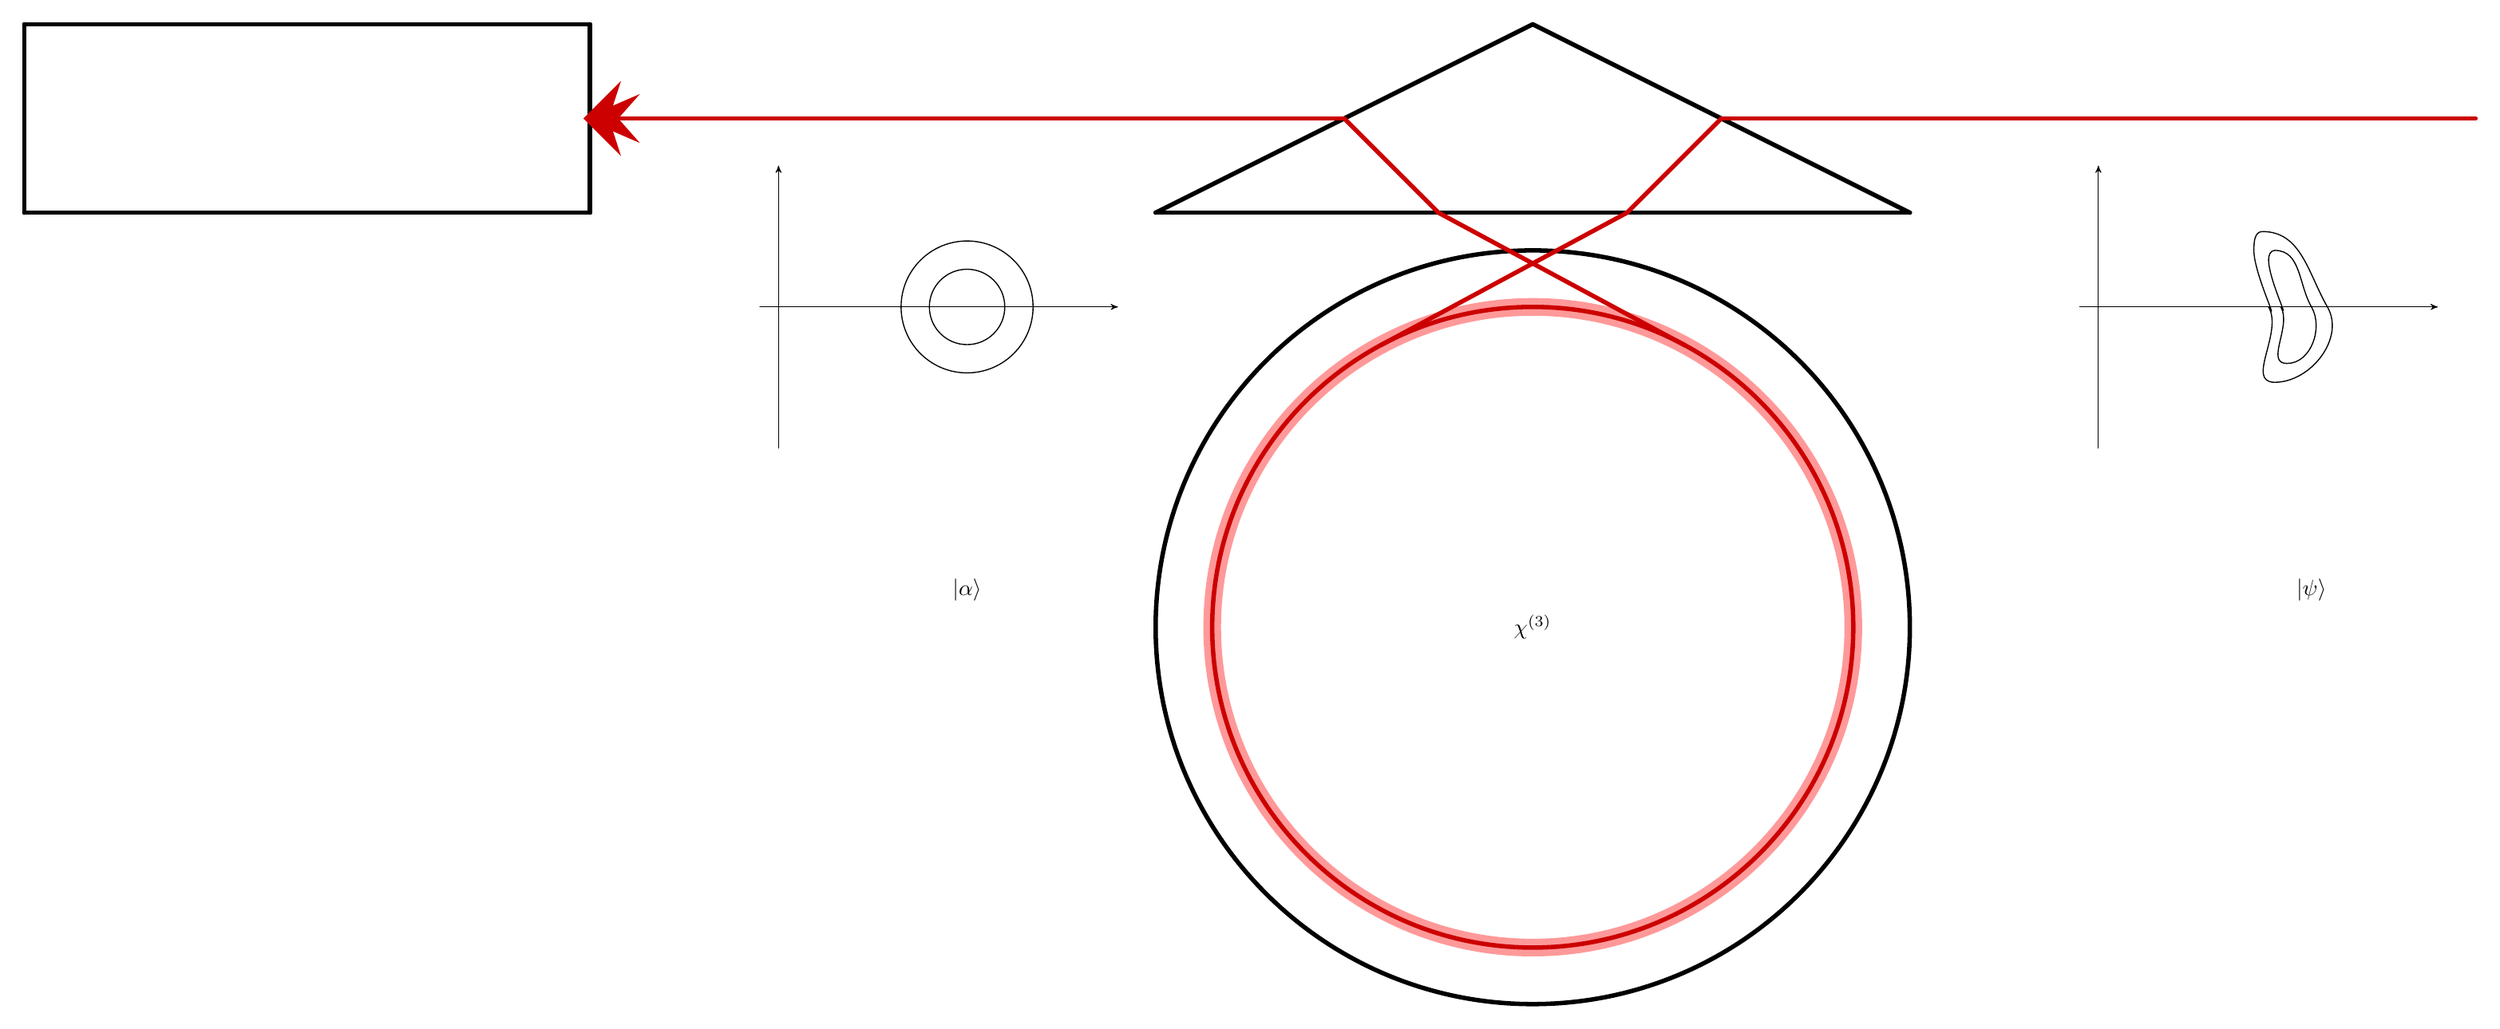
\begin{tikzpicture}[line cap=round,line join=round,>=triangle 45,x=1cm,y=1cm, 
    axis/.style={line width= 0.3pt, ->, >=stealth'}, scale=3]
% \clip(-5.208032545829854,-6.506121870314113) rectangle (15.714449254128738,6.275612465660563);
\definecolor{ccqqqq}{rgb}{0.8,0,0}
\definecolor{lightred}{rgb}{1,0.6,0.6}
\def\scal{0.65}
% rect
\draw [line width=2pt] (0,0) -- (3,0);
\draw [line width=2pt] (3,1) -- (3,0);
\draw [line width=2pt] (3,1) -- (0,1);
\draw [line width=2pt] (0,1) -- (0,0);
% triang
\def\lev{0.5}
\def\v{0.5}
\draw [line width=2pt] (6,\lev-\v)-- (10,\lev-\v);
\draw [line width=2pt] (8,\lev+\v)-- (10,\lev-\v);
\draw [line width=2pt] (8,\lev+\v)-- (6,\lev-\v);
% horisontal laser
\draw [line width=2pt,color=ccqqqq] (3,\lev) -- (7,\lev);
\draw [line width=2pt,color=ccqqqq] (9,\lev) -- (13,\lev);
% nonhorizontal in triangle
\draw [line width=2pt,color=ccqqqq] (7,\lev) -- (7.5,\lev-\v);
\draw [line width=2pt,color=ccqqqq] (9,\lev) -- (8.5,\lev-\v);
% resonator
\def\centy{\lev-2.7}
\draw [line width=2pt] (8,\centy) circle (2);
% lines in resonator
% circle
\draw [line width=8pt,color=lightred] (8,\centy) circle (1.7);
\draw [line width=2pt,color=ccqqqq] (8,\centy) circle (1.7);
% tangent line
\draw [line width=2pt,color=ccqqqq] (7.5,\lev-\v) -- (8.805956084154726, -0.7031917990557444);
\draw [line width=2pt,color=ccqqqq] (8.5,\lev-\v) -- (7.194043915845274, -0.7031917990557441);
% laser
\fill [ccqqqq] (3cm - 1pt,\lev) -- ++(0.2, 0.2) -- (3+0.1,\lev);
\fill [ccqqqq] (3cm - 1pt,\lev) -- ++(+0.2, -0.2) -- (3+0.1,\lev);
\fill [ccqqqq] (3cm - 1pt,\lev) -- ++(0.3, 0.13) -- (3+0.15,\lev);
\fill [ccqqqq] (3cm - 1pt,\lev) -- ++(+0.3, -0.13) -- (3+0.15,\lev);
% TEXT
% chi (3)
\node[] at (5,\lev-2.5) {$\ket{\alpha}$};
\node[] at (5+7+0.2*\scal,\lev-2.5) {$\ket{\psi}$};
\node[align=center] at (8,\centy) {$\chi^{(3)}$};
% Axis
\draw[axis] (4-0.1, \lev - 1) -- (5.8, \lev - 1) node(xline)[right]{};
\draw[axis] (4, \lev - 1.75) -- (4, \lev - 0.25) node(yline)[above] {};
\draw[axis] (4-0.1 + 7, \lev - 1) -- (5.8+7, \lev - 1) node(xline)[right]{};
\draw[axis] (4+7, \lev - 1.75) -- (4+7, \lev - 0.25) node(yline)[above] {};
% Plot circles
\draw [line width=0.5pt] (5,\lev - 1) circle (0.35);
\draw [line width=0.5pt] (5,\lev - 1) circle (0.2);
% Plot curves
\draw[line width=0.5pt] (5+7+0.2*\scal, \lev - 1) to [out=120, in=0] ++(-0.2*\scal - 0.1*\scal, + 0.3)
    to [out=180, in=90] ++ (-0.05*\scal, -0.05)
    to [out=270, in=300] (5+7-0.05*\scal, \lev - 1)
    to [out=300, in=180] (5+7, \lev-1 - 0.3)
    to [out=0, in=300] (5+7+0.2*\scal, \lev - 1);
\draw[line width=0.5pt] (5+7+0.33*\scal, \lev - 1) to [out=120, in=0] ++(-0.33*\scal - 0.2*\scal, + 0.4)
    to [out=180, in=90] ++ (-0.07*\scal, -0.1)
    to [out=270, in=300] (5+7-0.15*\scal, \lev - 1)
    to [out=300, in=180] (5+7-0.1*\scal, \lev-1 - 0.4)
    to [out=0, in=300] (5+7+0.33*\scal, \lev - 1);
\end{tikzpicture}
    \end{center}
}
\end{columns}

\begin{columns}
    \column{0.5}
    \block{Wigner calculation}
    {
        \begin{eqw}
            O(1+\abs{\alpha\Gamma})\\
            \abs{\alpha}^2 \gtrsim \Gamma^{-2}
        \end{eqw}
        \begin{eqw}
            \Gamma = 2\pi \frac{k}{n}
        \end{eqw}
        We use the interesting fact:\\
        \begin{align*}
            \frac{dF}{dA}(A, e^{i\Gamma}) = e^{i\Gamma} F(Ae^{2i\Gamma}, e^{i\Gamma})
        \end{align*}
        So we find an alternative repr for F for $\Gamma = 2\pi \frac{k}{n}$:\\
        \begin{align}
           F(A, e^{i\Gamma}) = \frac{\sum_{j\in\groupn}\exp\left(-i\Gamma j^2 + A e^{2ij\Gamma}\right)}{\sum_{j\in\groupn}\exp\left(-i\Gamma j^2\right)}
        \end{align}
        picture with some peaks\\
        Then using characteristic functions connection and finding a lot of Gaussian integrals we find:\\
        \begin{eqw*}
            W(\beta) &= \frac{2}{\pi}e^{\abs{\alpha}^2 - 2\left(\abs{\alpha} - \abs{\beta}\right)^2}\sum\limits_{m=0}^{\infty} \frac{\left(-|\alpha|^2\right)^m}{m!}\left|F(2\alpha \beta^* e^{i\Gamma(2m-1)}, e^{i\Gamma})e^{-2\abs{\alpha\beta^*}}\right|^2\\
            W(\beta) &= 2e^{2|\beta|^2}\sum\limits_{m=0}^{\infty} \frac{\left(-|\alpha|^2\right)^m}{m!}Q(2\beta e^{-i\Gamma 2m})
        \end{eqw*}
        the work in this direction is in progress
    }

    \column{0.5}
    \block{Husimi calculation}
    {
        Firstly we rewrite the expression for $F$ using integral:\\
        \begin{eqw}
            \Gamma = \frac{\pi}{6}\\
            \sum\limits_{n=0}^{\infty} \frac{A^n e^{i\Gamma n^2}}{n!} = \frac{e^{i\frac{\pi}{4}\sign \Gamma}}{2\sqrt{\pi|\Gamma|}}
            \int\limits_{-\infty}^{\infty} \exp\left(-\frac{z^2}{4\Gamma} + i A z\right) dz
        \end{eqw}
        then we deform the integration contour:
        \begin{center}
            \begin{tikzfigure}
                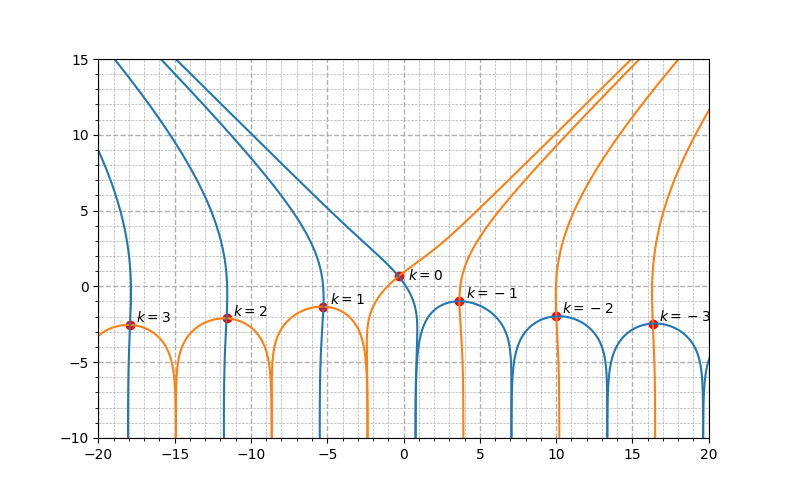
\includegraphics[width=0.45\textwidth]{v.png}
            \end{tikzfigure}
        \end{center}
        we use the method of steepest descent:
        \begin{eqw}
            \int\exp\left(f(z)\right)dz = \sum\limits_{k} \int\limits_{\gamma_k} \exp\left(f(z)\right)dz \approx
            \sum\limits_k \exp\left(f(z_k)\right)\sqrt{\frac{2\pi}{-f''(z_k)}}
        \end{eqw}
        concluding, we find the asymptotic expr for $F$:\\
        \begin{eqw*}
            \sum\limits_{n=0}^{\infty}\frac{A^n e^{i\Gamma n^2}}{n!} &\approx e^{\frac{i\pi}{4}\sign\Gamma}
            \frac{\exp\left(\frac{-i+i( W_{\bar k}(-2i A\Gamma)+1)^2}{4\Gamma}\right)}
            {\sqrt{-i\sign \Gamma\left(1+W_{\bar k}(-2i A\Gamma)\right)}}\\
            \bar k&\approx -\sign \Gamma \left[ \frac{2\abs{A\Gamma} + \left|\arg A\right|}{2\pi}\right]
        \end{eqw*}
        where we've hidden bulky remainder.\\
        pics with Q for 2 different alpha and gamma: small like banana and big which we've achived
    }
\end{columns}

\end{document}
